\documentclass[12pt,a4paper]{report}


\usepackage{amsmath}
\usepackage[utf8]{inputenc}
\usepackage{amsmath}
\usepackage{amsfonts}
\usepackage{amssymb}
\usepackage{calrsfs}
\usepackage[left=2cm,right=2cm,top=2cm,bottom=2cm]{geometry}
\usepackage[mathscr]{euscript}
\usepackage{graphicx}
\usepackage{tikz} %for drawing diagrams
\usetikzlibrary{arrows,shapes,trees}
%\usepackage{mathrsfs}

%%%%%%%%%for adding margins%%%%%%%%%
\usepackage{scrextend}
%%%%%%%%%%%%%%%%%%%%%%%%%%%%%%%

%%%%%%%%%%for writing large parallel%%%%%%
\usepackage{mathtools}
\DeclarePairedDelimiter\bignorm{\lVert}{\rVert}
%%%%%%%%%%%%%%%%%%%%%%%%%%%%%%%%%%%%%%%%%%

%for drawing commutative diagrams.
\usepackage{tikz-cd}  
%%%%%%%%%%%%%%%%%%%%%%%%%%%


%%%%%%%%%%%for wide hat%%%%%%%%%%%%
\usepackage{scalerel,stackengine}
\stackMath
\newcommand\reallywidehat[1]{%
\savestack{\tmpbox}{\stretchto{%
  \scaleto{%
    \scalerel*[\widthof{\ensuremath{#1}}]{\kern-.6pt\bigwedge\kern-.6pt}%
    {\rule[-\textheight/2]{1ex}{\textheight}}%WIDTH-LIMITED BIG WEDGE
  }{\textheight}% 
}{0.5ex}}%
\stackon[1pt]{#1}{\tmpbox}%
}

%\renewcommand{\hat}{\reallywidehat}
%%%%%%%%%%%%%%%%%%%%%%%%%%%%%%%%%%
\renewcommand{\hat}{\widehat}


%%%%%%%%%%for changing margin
\def\changemargin#1#2{\list{}{\rightmargin#2\leftmargin#1}\item[]}
\let\endchangemargin=\endlist 

\newenvironment{proof}
{\begin{changemargin}{1cm}{0.5cm}
	}%your text here
	{\end{changemargin}
}
\newenvironment{subproof}
{\begin{changemargin}{0.5cm}{0.5cm}
	}%your text here
	{\end{changemargin}
}
%%%%%%%%%%%%%%%%%%%%%%%%%%%%%

\usepackage{empheq}
%%%%%%%%%%for writing symbol above an equality
\newcommand{\xeq}[1]{\stackrel{\mathclap{\normalfont\mbox{\tiny{#1}}}}{=}}
%%%%%%%%%%%%%%%%%%%%%%%%%%%%%%%%%%%%%%%%%%%%


%%%%%%%%%%%%%%double rules%%%%%%%%%%%%%%%%%%%
\usepackage{lipsum}% Just for this example

\newcommand{\doublerule}[1][.4pt]{%
  \noindent
  \makebox[0pt][l]{\rule[.7ex]{\linewidth}{#1}}%
  \rule[.3ex]{\linewidth}{#1}}
%%%%%%%%%%%%%%%%%%%%%%%%%%%%%%%%%%%%%%%%%%%%%%


\begin{document}
\newcommand{\thm}{\textbf{Theorem) }}
\newcommand{\thmnum}[1]{\textbf{Theorem #1) }}
\newcommand{\defi}{\textbf{Definition) }}
\newcommand{\lem}{\textbf{Lemma) }}
\newcommand{\lemnum}[1]{\textbf{Lemma #1) }}
\newcommand{\prop}{\textbf{Proposition) }}
\newcommand{\propnum}[1]{\textbf{Proposition #1) }}
\newcommand{\cor}{\textbf{Corollary) }}
\newcommand{\cornum}[1]{\textbf{Corollary #1) }}


\newcommand{\pf}{\textbf{proof) }}
\newcommand{\eop}{\hfill  \textsl{(End of proof)} $\square$} %end of proof


\newcommand{\lap}{\triangle} %%Laplacian
\newcommand{\s}{\vspace{10pt}}
\newcommand{\bull}{$\bullet$}
\newcommand{\sta}{$\star$}
\newcommand{\reals}{\mathbb{R}}

\newcommand{\intN}{\mathbb{Z}_N}
\newcommand{\norms}[2]{\bignorm[\big]{#1}_{#2}}
\newcommand{\avg}{\mathbb{E}}
\newcommand{\prob}{\mathbb{P}}
\newcommand{\osc}{\text{\osc}}

\renewcommand{\P}{\mathscr{P}}

%\renewcommand{\choose}[2]{\scalebox{0.5}{\begin{pmatrix}
%#1 \\
%#2
%\end{pmatrix}}}

%%%%%%%box norms%%%%%%%%%%%%%%%%%%%%%%%%%%%%%%%%%%%%
\newcommand{\boxnorm}[1]{\norms{#1}{\tiny{\square}}}
\newcommand{\boxinn}[4]{\begin{array}{|cc|} 
\cline{1-2}
#1 & #2 \\
#3 & #4 \\
\cline{1-2}
\end{array}}
%%%%%%%%%%%%%%%%%%%%%%%%%%%%%%%%%%%%%%%%%%%%%%%%%%%%%%

\newcommand{\newday}{\doublerule[0.5pt]}
%\newcommand{\newday}{================================================================}
\newcommand{\digression}{**********************************************************************************************}

\renewcommand{\bar}{\overline}

\setlength\parindent{0pt}

\chapter*{Combinatorics}
\s

Lecturer : Prof. Imre Leader
\s


\section*{Chapter 3. Projections}
``If a set has small projections, must it be small?"

\begin{itemize}
\item Let $A\subset \P(X)$. For $Y\subset X$, the \textbf{projection} or \textbf{trace} of $A$ on $Y$ is
\begin{align*}
A| Y = \{x\cap Y : x\in A \}
\end{align*}
``project $A$ on the coordinates corresponding to $Y$"

e.g. if $A = \{14,25,26,127,128\}$, then $A |\{1,2\} = \{1,2,12\}$ so $A|Y \subset \P(Y)$.
\item Say $A$ \textbf{covers} or \textbf{shatters} $Y$ if $A|Y = \P(Y)$.
\item The \textbf{trace number} or \textbf{VC-dimension} of $A$ is (V : Vapnik, C : Cernovnkis)
\begin{align*}
\text{tr}(A) = \max \{|Y|: A \text{ shatters } Y \}
\end{align*}
\end{itemize}
\s

Given $|A|$, how small can tr($A$) be?

\quad Equivalentely, if tr($A$)<$k$(i.e. $A$ does not shatter any $k$-set), how large can $A$ be?
\begin{itemize}
\item Trivially, must have $|A| \leq (1-2^{-k})2^n$ (else $A$ shatter every $k$-set)
\item Could take $A= X^{(<k)}$-no $k$-set $Y$ is shattered, as $Y \not\in A|Y$.
\end{itemize}
\s

\textbf{Aim :} $A = X^{(<k)}$ is the best
\s

\textit{Remark :} very striking as from each $k$-projection having size $\leq(1-2^{-k})$, total we are getting a very small (polynomial in $n$) bound on $|A|$.
\s

\textit{Idea :} trivial that $|A| \leq |X^{(<k)}|$ if $A$ is a \textbf{down set}(i.e. if $x\in A$ and $y\subset x$ then $y\in x$). Indeed, must have $A\subset X^{(<k)}$, since if $A$ contains a set $x$ with $|x|\geq k$ then $A|x = \P (x)$. So ``try to make $A$ into a down-set".
\s

For $A \subset \P(X)$ and $1\leq i\leq n$ the \textbf{$i$-down-compression} of $A$ is defined as follows :
\begin{proof}
for $x\in \P(x)$, set
\begin{align*}
D_i(x) = \begin{cases}
\begin{array}{ll}
x & \text{if } i \not\in x \\
x- \{i\} & \text{if } i\in x
\end{array}
\end{cases}
\end{align*}
and set $D_i(A) = \{D_i(x) : x\in A \} \cup \{x\in A : D_i(x)\in A\}$. ``remove element $i$ whenever possible".
\end{proof}
\s

\thmnum{1} \emph{(Sauer-Shelah lemma)} Let $A\subset \P(X)$ with $\text{tr}(A) <k$. Then $|A| \leq |X^{(<k)}|$.
\begin{proof}
\pf Given $1\leq i\leq n$,

\textit{Claim :} $\text{tr}(D_i(A)) \leq \text{tr}(A)$.
\begin{subproof}
\pf Write $B= D_i(A)$ - we'll show that if $B$ shatters $Y$ (some $Y$) then $A$ shatters $Y$.

If $i\not\in Y$< then $B|Y = A|Y$, so may assume $i\in Y$. Given $z\subset Y$ with $i\not\in z$, we'll show $z$, $z\cup \{i\} \in A|Y$. Since $z\cup \{i\} \in B|Y$, have $z\cup \{i\} \cup x \in B$, some $x \subset X \backslash Y$. Hence $z\cup x$ and $z\cup\{i\}\cup x\in A$ (by definition of $D_i$) whence $z$, $z\cup \{i\} \in A|Y$.
\end{subproof}
Now let $D = D_n(D_{n-1}(\cdots D_1(A) \cdots))$. Then $|D|=|A|$, $D$ is a down-set and $\text{tr}(D) \leq \text{tr}(A) <k$. Thus $|D| \leq |X^{(<k)}|$.

\eop
\end{proof}
\s

\textit{Remark :} we used 1-dimensional compression.
\s

Now, we have : if all $k$-dimensional projections have size $\leq 2^k-1$, then $A$ is small ($|A| \leq \sum_{i=0}^{k-1} {n \choose k}$)
\s

What about other bounds? For example, what if each $k$-dimensional projection is $\leq \frac{1}{2}$-sized ($\big| A|Y \big| \leq 2^{k-1}$?)
\s

\begin{itemize}
\item A \textbf{box} or \textbf{brick} in $\reals^n$ is a set of the form $[a_1,b_1] \times \cdots \times [a_n, b_n]$, where $a_i \leq b_i$ for all $i$. 
\item A \textbf{body} $S\subset \reals^n$ is a \emph{finite union} of bricks. For $S$ a body, write $|S|$ or $m(S)$ for the volume of $S$. 
\end{itemize}
\s

\textit{Remarks :}
\begin{itemize}
\item[1.] Everything unchanged if we only assume $S$ compact (or just bounded and measurable)
\item[2. ] For $A\subset \P(X) \leftrightarrow \{0,1\}^n$, have corresponding body $\hat{A} \subset \reals^n$ with $m(\hat{A}) = |A|$, namely :
\begin{align*}
\hat{A} = \cup_{x\in A} [x_1, x_1 +1] \times \cdots \times [x_n, x_n +1]
\end{align*} 
\end{itemize}
\s

For body $S\subset \reals^n$ and $Y\subset \{1,2\cdots, n\}$, write $S_Y$ for the projection of $S$ onto the subspace spanned by the $e_i$, $i\in Y$.

\textit{e.g.} for $S\subset \reals^3$, $S_1$ is the projection of $S$ onto the $x$-axis. i.e. $S_1 = \{x_1 : (x_1, x_2, x_3) \in S$, some $x_2, x_3 \}$. $S_{12}$ is the projection of $S$ onto the $xy$-plane, i.e. $S_{12} = \{(x_1, x_2) : (x_1, x_2, x_3) \in S$ some $x_3 \}$.
\s

\textbf{Question :} When do an upper bound of $|S|$ exist given the values of $S_Y$?
\s

\textit{e.g.}
\begin{itemize}
\item for $S\subset \reals^3$, $|S|\leq |S_1||S_2||S_3|$, as $S\subset S_1\times S_2\times S_3$. Also, $|S|\leq |S_{12}||S_3|$, as $S\subset S_{12} \times S_3$.
\item But $\{|S_{12}|,S_{13}\}$ does not bound $|S|$, e.g. $S = [0, \frac{1}{N}]\times [0,N]\times [0,N]$.
\item How about $\{|S_{12}|, |S_{23}|,|S_{13}|\}$?
\end{itemize}
\s

\propnum{2} Let $S$ be a body in $\reals^3$. Then $|S|^2 \leq |S_{12}||S_{23}||S_{13}|$.
\s

\textit{Notes} 
\begin{itemize}
\item[1.] Can have equality, e.g. when $S$ is a brick
\item[2.] For $S\subset \reals^n$, the \textbf{sections} of $S$ are the sets $S(x) \subset \reals^{n-1}$($x\in \reals)$ given by
\begin{align*}
S(x) = \{(x_1, \cdots, x_{n-1})\in \reals^{n-1} : (x_1, \cdots, x_{n-1},x)\in S \}
\end{align*}
\end{itemize}
\begin{proof}
\pf Suppose first that every section of $S$ is a square, $S(x) = [0, f(x)] \times [0, f(x)]$ for all $x$. Then $|S_{12}| = M^2$, where $M= \max_{x} f(x)$. Also $|S_{13}| = |S_{23}| = \int f(x) dx$. So want : $(\int f^2)^2 \leq M^2 (\int f)^2$, i.e. $\int f^2 \leq M \int f$, which is true because $f(x)^2 \leq M f(x)$ for all $x$.
\s

For general $S$, \emph{define} body $T\subset \reals^3$ by giving its sections,
\begin{align*}
T(x) = [0, \sqrt{|S(x)|}] \times [0, \sqrt{|S(x)|}]
\end{align*}
so $|T| = |S|$. Certainly have $|T_{12}| \leq |S_{12}|$, since $|T_{12}| \leq \max_x |T(x)|$.

\quad Write $g(x) = |S(x)_1|$, $h(x) = |S(x)_2|$, so $|S(x)| \leq g(x) h(x)$. Have $|S_{13}| = \int g(x) dx$ and $|S_{23}|= \int h(x) dx$. Also, 
\begin{align*}
T_{13}|=|T_{23}| &= \int \sqrt{|S(x)|} dx \leq \int \sqrt{g(x)h(x)}dx \\
&\leq (\int g)^{1/2} (\int h)^{1/2} \quad \text{(Cauchy-Schwarz)}
\end{align*}

\eop
\end{proof}
\s

\begin{itemize}
\item Sets $Y_1, \cdots, Y_r \subset[n]$ \textbf{cover} $[n]$ if $Y_1\cup \cdots \cup Y_r =[n]$. They are a \textbf{k-uniform cover} if each $i\in [n]$ belong to exactly $k$ of $Y_1, \cdots, Y_r$.

\textit{e.g.} $\{1\},\{2\},\{3\}$ is a 1-uniform cover of [3]. $\{1\},\{2,3\}$ is a 1-uniform cover of [3]. $\{1,2\}, \{1,3\}$ is not a uniform cover of [3]. $\{1,2\},\{2,3\},\{1,3\}$ is a 2-uniform cover of [3].
\s
\end{itemize}
\s

\textbf{Aim :} $|S|^k \leq |S_{Y_1}| \cdots |S_{Y_r}|$ where $Y_1, \cdots, Y_r$ is a $k$-uniform cover of $[n]$.
\s

\newpage

\newday

(29th November, Thursday)
\s

(3rd example class is at 5pm Thursday, 24th - hand in Q1,5,6, directly to the pigeon hole)

\subsubsection*{Intersecting Families of Graphs}

So far, for $n$ families, our object lived in $[n]$(no structure). What if the ground set has some structure?
\s

For example, ground set$=[n]^{(2)}=$edges of a graph on $[n]$=subgraphs of $H_n$, there are $2^{n(n-1)/2}$ possible graphs.
\s

Let $A \subset \mathscr{P}([n]^{(2)})$ be a family of graphs on $n$ vertices. For any fixed graph $H$, we say $A$ is \textbf{$H$-intersecting} if $\forall G, G' \in A$, $G\cap G'$ contains a copy of $H$ ("$G\cap G' \supset H$")

\textit{e.g.} $H=P_1$=single edge. Then $A$ is $H$-intersecting implies that $|A| \leq \frac{1}{2} 2^{n(n-1)/2}$ (as cannot have both $G, G^c \in A$) and can achieve this, e.g. $A =\{G : 12\in G\}$. (indeed, for any $H$ (non-empty), $A$ being $H$-intersecting implies $|A| \leq \frac{1}{2}2^{n(n-1)/2})$.
\s

What about $H=P_2$? ($P_2=$ 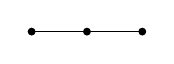
\begin{tikzpicture}
\fill[black] (0,0) circle (0.05);
\draw (0pt,0pt) -- (20pt,0pt);
\fill[black] (20pt,0) circle (0.05);
\draw (20pt, 0) -- (40pt, 0pt);
\fill[black] (40pt,0) circle (0.05);
\end{tikzpicture})
\begin{proof}
Obvious guess is $A = \{G: G$ contains $H_0 \}$ where $H_0 = \{$some fixed copy of $P_2\}$, e.g. $H_0 =$ 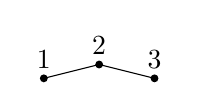
\begin{tikzpicture}
\path[draw] (0, 0) node[above]{1} -- (20pt,5pt) node[above]{2} -- (40pt,0) node[above]{3};
\fill[black] (0pt,0pt) circle (0.05);
\fill[black] (20pt,5pt) circle (0.05);
\fill[black] (40pt,0pt) circle (0.05);
\end{tikzpicture}. This has size $A= \frac{1}{4}2^{n(n-1)/2}$. But can do better : e.g. $A = \{G: d_G(1) \geq \frac{n}{2} +1 \}$ (where $d_G(1) =\#$ edges out of 1). This has
\begin{align*}
|A| = 2^{n(n-1)/2} (\frac{1}{2} -\frac{c}{\sqrt{n}}) = (\frac{1}{2} + o(1)) 2^{n(n-1)/2}
\end{align*}
i.e. tends to $\frac{1}{2}2^{n(n-1)/2}$
\end{proof}

\s

Similarly, if $H$ is any star \Big( 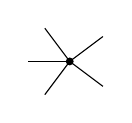
\begin{tikzpicture}
\fill[black] (0pt,0pt) circle (0.05);
\draw (0, 0) -- (12pt,9pt); \draw (0, 0) -- (12pt,-9pt);
\draw (0, 0) -- (-15pt,0pt);
\draw (0, 0) -- (-9pt,12pt);
\draw (0, 0) -- (-9pt,-12pt);
\end{tikzpicture} \Big), we have $H$-intersecting families of size $(\frac{1}{2} - o(1))2^{n(n-1)/2}$.
\s

How about $\triangle$-intersecting ($\triangle$=triangle) ?
\begin{proof}
Obvious guess is $|A| = \frac{1}{8} 2^{n(n-1)/2}$ ($A= \{G: G \supset$ fixed triangles $\}$)
\end{proof}
\s

\textbf{Simonovits-Sos conjecture :} If $A$ is $\triangle$-intersecting, then $|A| \leq \frac{1}{8}2^{n(n-1)/2}$.
\s

\thmnum{8} Let $A\subset \mathscr{P}([n]^{(2)})$ be $\triangle$-intersecting. Then $|A| \leq \frac{1}{4}2^{n(n-1)/2}$.
\begin{proof}
\pf Say $n$ is even.

\quad Consider the projection of $A$ onto the edge-set $Y= B^{(2)} \cup (B^c)^{(2)}$, any $B\subset [n]$, $B= n/2$. then $G, G' \in A$ implies $G\cap G'$ must meet $Y$. (Because every triangle meets $Y$). Thus $A|Y$ is an intersecting family of sets. So
\begin{align*}
\big| A|Y \big| \leq \frac{1}{2} 2^{2 {n/2 \choose 2} } = 2^{2 {n/2 \choose 2} (1- \frac{1}{2 {n/2 \choose 2}}) }
\end{align*}
But the $Y$ form a uniform cover of $[n]^{(2)}$ (as $B$ varies) so by \textbf{Corollary 5}, have
\begin{align*}
|A| \leq 2^{2 {n/2 \choose 2} } = 2^{ {n/2 \choose 2} (1- \frac{1}{2 {n/2 \choose 2}}) }
\end{align*}
so done if
\begin{align*}
\begin{pmatrix}
n \\
2
\end{pmatrix} (1- \frac{1}{2 {n/2 \choose 2}}) \geq 2
\end{align*}
But (\textbf{LHS})=$\frac{n(n-1)}{2\cdot \frac{n}{2}\cdot (\frac{n}{2}-1)} = \frac{n-1}{\frac{n}{2}-1} >2$, so done.
\s

For $n$ odd, the proof is same with $|B| = \frac{n-1}{2}$

\eop
\end{proof}
\s

Simonovits-Sos conjecture was proved in 2010 (Ellis, Filmu, Friedent)
\s

Say $H$ \textbf{common} if $\max \{ |A| : A\subset \mathscr{P}([n]^{(2)})$ is $H$-intersecting$\}=(\frac{1}{2}- o(1))2^{n(n-1)/2}$.

\textit{e.g.} every star is commnon, $\triangle$ is not common. Any disjoint union of stars is also common, \textit{e.g.} take $n$ very large, $k$ large and
\begin{align*}
A = \{G : \text{at least } \frac{k}{2} +3 \text{ of vertices } 1, \cdots k \text{ have degree} \geq \frac{n}{2} + 5\}
\end{align*}
\s

\textbf{Key question :} is $P_3$(= 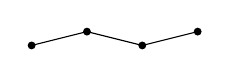
\begin{tikzpicture}
\path[draw] (0, 0)  -- (20pt,5pt) -- (40pt,0) -- (60pt, 5pt);
\fill[black] (0pt,0pt) circle (0.05);
\fill[black] (20pt,5pt) circle (0.05);
\fill[black] (40pt,0pt) circle (0.05);
\fill[black] (60pt,5pt) circle (0.05);
\end{tikzpicture}) common?

\quad This is an open question!
\s

\textbf{Easy fact :} every $G$, not a union of stars, contains $\triangle$ or $P_3$.
\s

So if we know $P_3$ not common, we would also know -
\s

\textbf{Alon's common graphs conjecture :} $H$ is common $\Leftrightarrow$ $H$ is a union of stars.
\s

\textit{But :} Christofides (2008) gave a $P_3$-intersecting family with density $\frac{17}{128} > \frac{1}{8}$.



\end{document}